\chapter{Kinematics}
The manipulator used was a four degree of freedom (DOF) arm with a gripper attached as the end effector. All joints were revolute and implemented by servo motors. A drawing of the arm is shown in Figure \ref{fig:ARM}. To properly control the manipulator the forward and inverse kinematics were derived.

\begin{figure} [h]
\centering
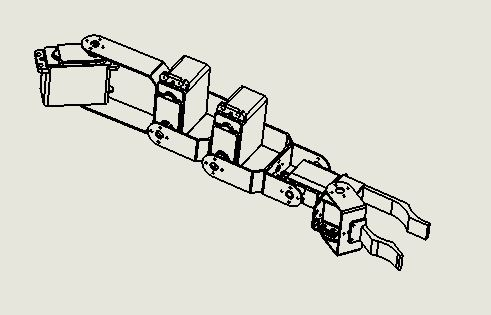
\includegraphics[width=0.5\textwidth]{armdrawing}
\caption{The Mobile Manipulator}
\label{fig:ARM}
\end{figure}

\section{Forward Kinematics}
Forward kinematics is finding the position and orientation of a manipulator's end effector given the position of all of its joints. For this manipulator the end effector position was calculated in terms of the angles of the first four joints of the manipulator $\theta_1$ - $\theta_4$. The gripper was considered only as a length as it has no effect on the arm's overall position or orientation. An manipulator simplified as a drawing of its joints can be seen in Figure \ref{fig:ARMCoord}.

\begin{figure}
\centering
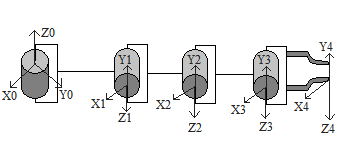
\includegraphics[width=0.5\textwidth]{manipulatoraxis}
\caption{The Mobile Manipulator with Coordinate Frames}
\label{fig:ARMCoord}
\end{figure}

The coordinate frames of each of the joints were found using the Devavit-Hartenberg (D-H) convention. The resulting coordinate frames and DH parameters are also drawn in Figure \ref{fig:ARMCoord}. The D-H table, which contains each of the D-H parameters for calculating the transformation matrix of each joint is shown in Table 1. The matrix for each joint was then calculated using the formula in equation \ref{eq:Amat} where $A_i$ is the transformation matrix between the coordinate frame $o_ix_iy_iz_i$ and $o_{i-1}x_{i-1}y_{i-1}z_{i-1}$ where $o_0x_0y_0z_0$ is the origin coordinate frame. The transformation matrix $T_4^0$, to convert from the coordinate frame of the end effector to the coordinate frame of the origin is found by multiplying all of the A matrices together. So $T_4^0$ = $A_1*A_2*A_3*A_4$. The fourth column of this matrix represents the the 3-Dimensional (3D) coordinates of the manipulator's end effector with respect to the origin coordinate frame. $R_{14}$ is the x position $R_{24}$ is the y position and $R_{34}$ is the z position where R = $\begin{bmatrix}
  r_{11} & r_{12} & r_{13} & r_{14} \\
  r_{21} & r_{22} & r_{23} & r_{24}\\
  r_{31} & r_{32} & r_{33} & r_{34} \\
  r_{41} & r_{42} & r_{43} & r_{44}
 \end{bmatrix}$. This column then returns the equations for x, y, and z in terms of the angles $\theta_1$ - $\theta_4$. As these equations are very long the matrices above were calculated for each value and multiplied in code rather than writing out the equations.
\begin{table}
\centering
\begin{tabular}{| l | l | l | l | l |}
 		\hline
 		Joint & $d_i$ & $\alpha_i$ & $a_i$ & $\theta_i$ \\ \hline
 		1 & 0 & $-90^o$ & $l_1$ & $\theta_1*$\\ \hline
 		2 & 0 & $0^o$ & $l_2$ & $\theta_2*$\\ \hline
 		3 & 0 & $0^o$ & $l_3$ & $\theta_3*$\\ \hline
 		4 & 0 & $0^o$ & $l_4$ & $\theta_4*$\\ \hline
	\end{tabular}
	\label{table:DH}
	\caption{D-H table}
\end{table}

\begin{equation}
\label{eq:Amat}
\begin{bmatrix}
  cos\theta_i & -sin\theta_icos\alpha_i & sin\theta_isin\alpha_i & \alpha_icos\theta_i \\
  sin\theta_i & cos\theta_icos\alpha_i & -cos\theta_isin\alpha_i & \alpha_isin\theta_i\\
  0 & sin\alpha_i & cos\alpha_i & d_i \\
  0 & 0 & 0 & 1
 \end{bmatrix}
\end{equation}

\section{Inverse Kinematics}
The inverse kinematics of a manipulator are a way to calculated the position of each of the joints of a manipulator in terms of end effector position. The inverse kinematics of this manipulator were simple enough to be calculated analytically. The process of this is discussed below.

The last three angles of the manipulator $\theta_2$, $\theta_3$, and $\theta_4$ all lie within the same plane as each other. This plane's location in 3D space is determined by $\theta_1$ which only moves in the x-y plane. The projection of the arm onto the x-y plane is shown in Figure \ref{fig:xy} where $x_c$ and $y_c$ are the desired x and y coordinates of the end effector. From this drawing it is easy to see that $\theta_1$ can be calculated as the inverse tangent of $\frac{(x_c)}{y_c}$ or $\theta_1 = Atan2(x_c,y_c)$ where Atan2 is the inverse tangent function taking signs into consideration.

The remaining three angles can be projected into the plane formed by the z-axis and the plane determined by $\theta_1$ in the x-y axis. This is seen in Figure \ref{fig:z} where r = $\sqrt{x^2+y^2} - l_1$ which is the length of the projected manipulator on the x-y plane. Two equations can be found for $z_c$ and r using geometric properties on the projected image. Since only two equations can be found and there are three unknown variables the desired orientation of the end effector $\theta_c$ must be specified. The resulting three equations are shown in equation \ref{eq:Zproj}.

\begin{subequations}
\label{eq:Zproj}
	\begin{align}
	z_c = l_2sin\theta_2+l_3sin(\theta_2+\theta_3) + l_4sin\theta_c\qquad \\
	r = l_2cos\theta_2+l_3cos(\theta_2+\theta_3) + l_4cos\theta_c\qquad \\
	\theta_c = \theta_2 + \theta_3 + \theta_4 \qquad 
	\end{align}
\end{subequations}

\begin{figure}
    \centering
    \begin{subfigure}[b]{0.3\textwidth}
    	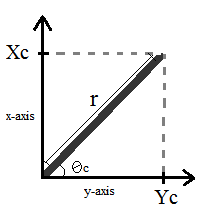
\includegraphics[width=\textwidth]{xyaxis}
    	\caption{Projection of Manipulator onto the XY axis}
   	 	\label{fig:xy}
   	 \end{subfigure}
   	 \quad
    \begin{subfigure}[b]{0.3\textwidth}
		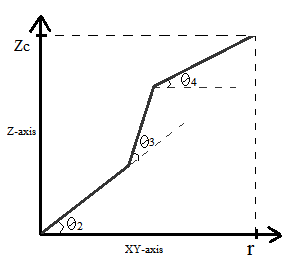
\includegraphics[width=\textwidth]{zprojection}
		\caption{Projection of Manipulator onto the Z-plane Axis. }
		\label{fig:z}
    \end{subfigure}
    \quad %add desired spacing between images, e. g. ~, \quad, \qquad, \hfill etc.
      %(or a blank line to force the subfigure onto a new line)
 	\caption{Projections for solving the inverse kinematics geometrically.}
\end{figure}
These equations were solved for $\theta_2$, $\theta_3$, and $\theta_4$.  The final results for the inverse kinematics; $\theta_1$, $\theta_2$, $\theta_3$, and $\theta_4$ in terms of $x_c$, $y_c$, $z_c$, and$\theta_c$ are shown in equation \ref{eq:inverse}.

\begin{subequations}
\label{eq:inverse}
	\begin{align}
	\theta_1 = Atan2(y_c,x_c)\qquad \\
	\theta_3 = cos^{-1}(\frac{(z_c-l_4sin\theta_c)^2+(r-l_4cos\theta_c)^2-l_2^2-l_3^2}{2l_2l_3})\qquad \\
	\theta_2 = tan^{-1}(frac{z_c-l_4sin\theta_c}{r-l_4cos\theta_c}) - tan^{-1}(frac{[l_3sin\theta_3],[l_2l_3cos\theta_3]}) \qquad \\
	\theta_4 = \theta_c - \theta_2 - \theta_3 \qquad
	r = \sqrt{x_c^2+y_c^2}-l_1
	\end{align}
\end{subequations}


It also becomes helpful to have a way to calculate if the increase kinematics is possible. If the calculation of $\theta_3$ is an imaginary number than there is no real solution to the inverse kinematics. Inverse cos returns an imaginary number when taking the inverse of a number greater than one. Therefore if the denominator is bigger than the numerator than the resulting $\theta_3$ will be imaginary. So if $(z_c-l_4sin(\theta_c))^2 + (r-l_4cos(\theta_c))^2 - l_2^2 - l_3^2) < 2l_2l_3$ than the desired x,y,z coordinates are outside of the workspace of the manipulator. 

The physical constraints of the manipulator must also be taken into account. Due to the way the arm is constructed the each joints has a limit of the angles it can be set to. The are as follows; $-90^o \leq \theta_1 \leq 90^o$, $-50^o \leq \theta_2 \leq 120^o$, $-55^o \leq \theta_3 \leq 120^o$, $-110^o \leq \theta_4 \leq 90^o$. These constraints were found by finding the angle at which the joints cannot turn farther without colliding with another part of the arm. A sample of the manipulator workspace taken at all possible angles with an increment of $5^o$ is shown in Figure \ref{fig:work}.  The code for handling the kinematics of the manipulator can be seen in Appendix B.5.

\begin{figure}
\centering
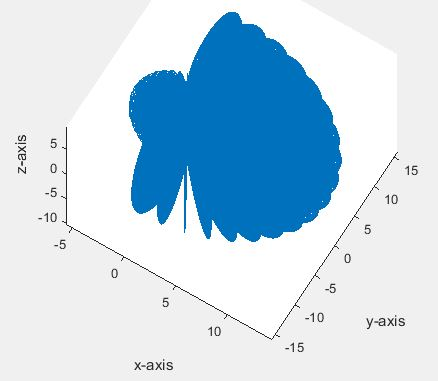
\includegraphics[width=0.5\textwidth]{workspace}
\caption{Workspace of the manipulator }
\label{fig:work}
\end{figure}